\section{Introduction to OpenPLC Editor} 

Creating, testing and executing ladder diagrams requires a PLC editor. OpenPLC Editor allows for writing PLC programs according to the IEC 61131-3 standard.

\subsection{Installing OpenPLC Editor}
OpenPLC Editor is installed in the ICSSecurity OVA available through the ICS Security GitHub. The directions for a clean installation can be found at https://www.openplcproject.com/plcopen-editor. Currently, the only two versions available for installation are for Windows and Linux.

\subsection{Opening OpenPLC Editor}
There are two ways to open the OpenPLC editor. 
\begin{itemize}[noitemsep]
    \item If you created a virtual machine from the provided OVA, there is an icon on the desktop. Clicking the icon will open the OpenPLC editor.
    \item Open a terminal and execute the following command ~/Downloads/OpenPLC\_Editor/openplc\_editor.sh 
\end{itemize}

The editor is divided into different quadrants. Figure~\ref{fig:editorEmpty} displays the editor without an open project. Figure~\ref{fig:editorProject} displays an open project containing variable declarations, the ladder diagram, configuration information, and a debugger window.

\clearpage
\begin{figure}[!htb]
\begin{center}
\tcbox[colframe=black,colback=white!30]{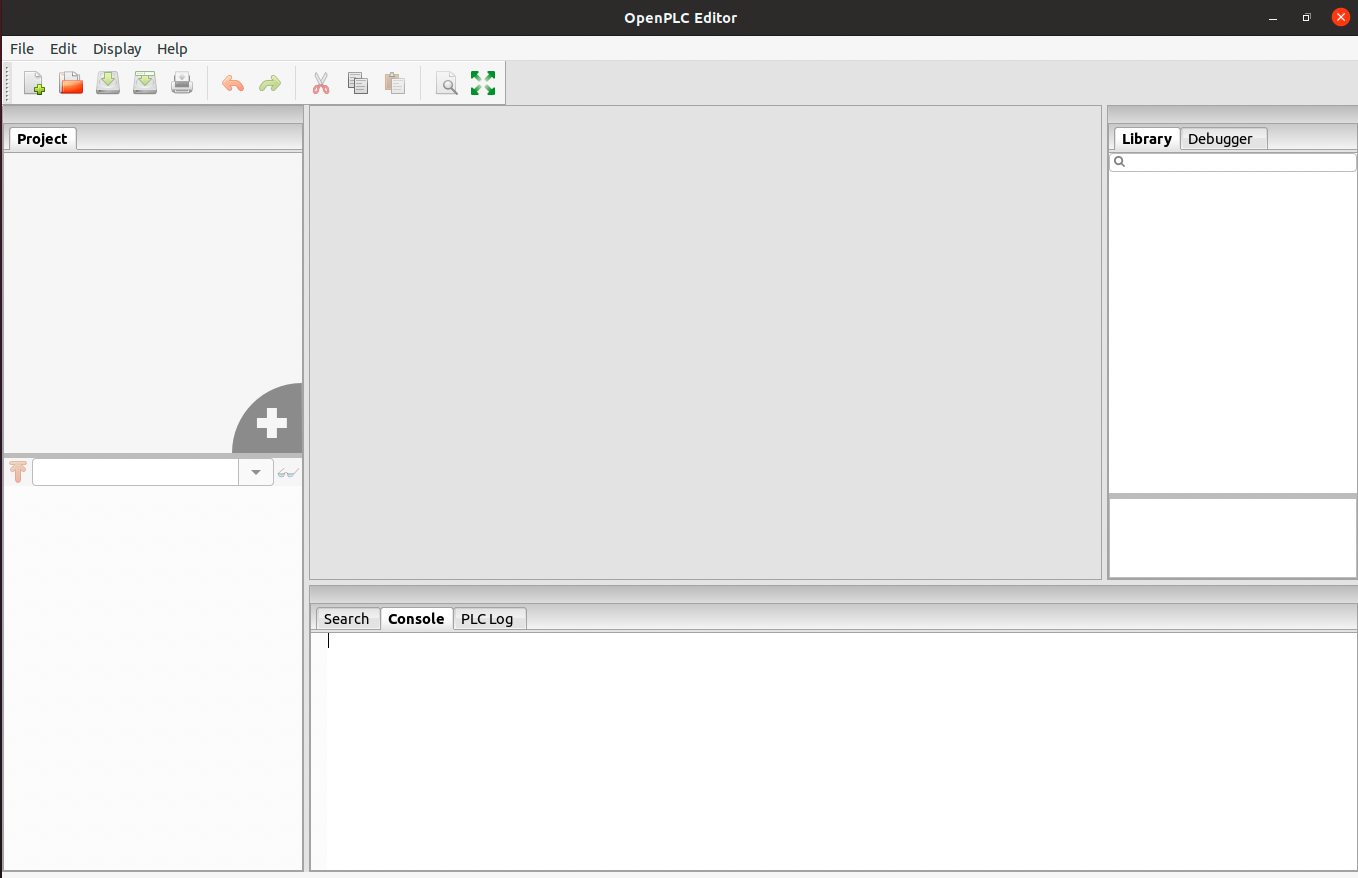
\includegraphics[width=.9\textwidth]{./images/editorEmpty.png}}
\end{center}
\caption{The OpenPLC Editor without a project or ladder diagram}
\label{fig:editorEmpty}
\end{figure}

%\hspace{3cm}
\begin{figure}[!htb]
\begin{center}
\tcbox[colframe=black,colback=white!30]{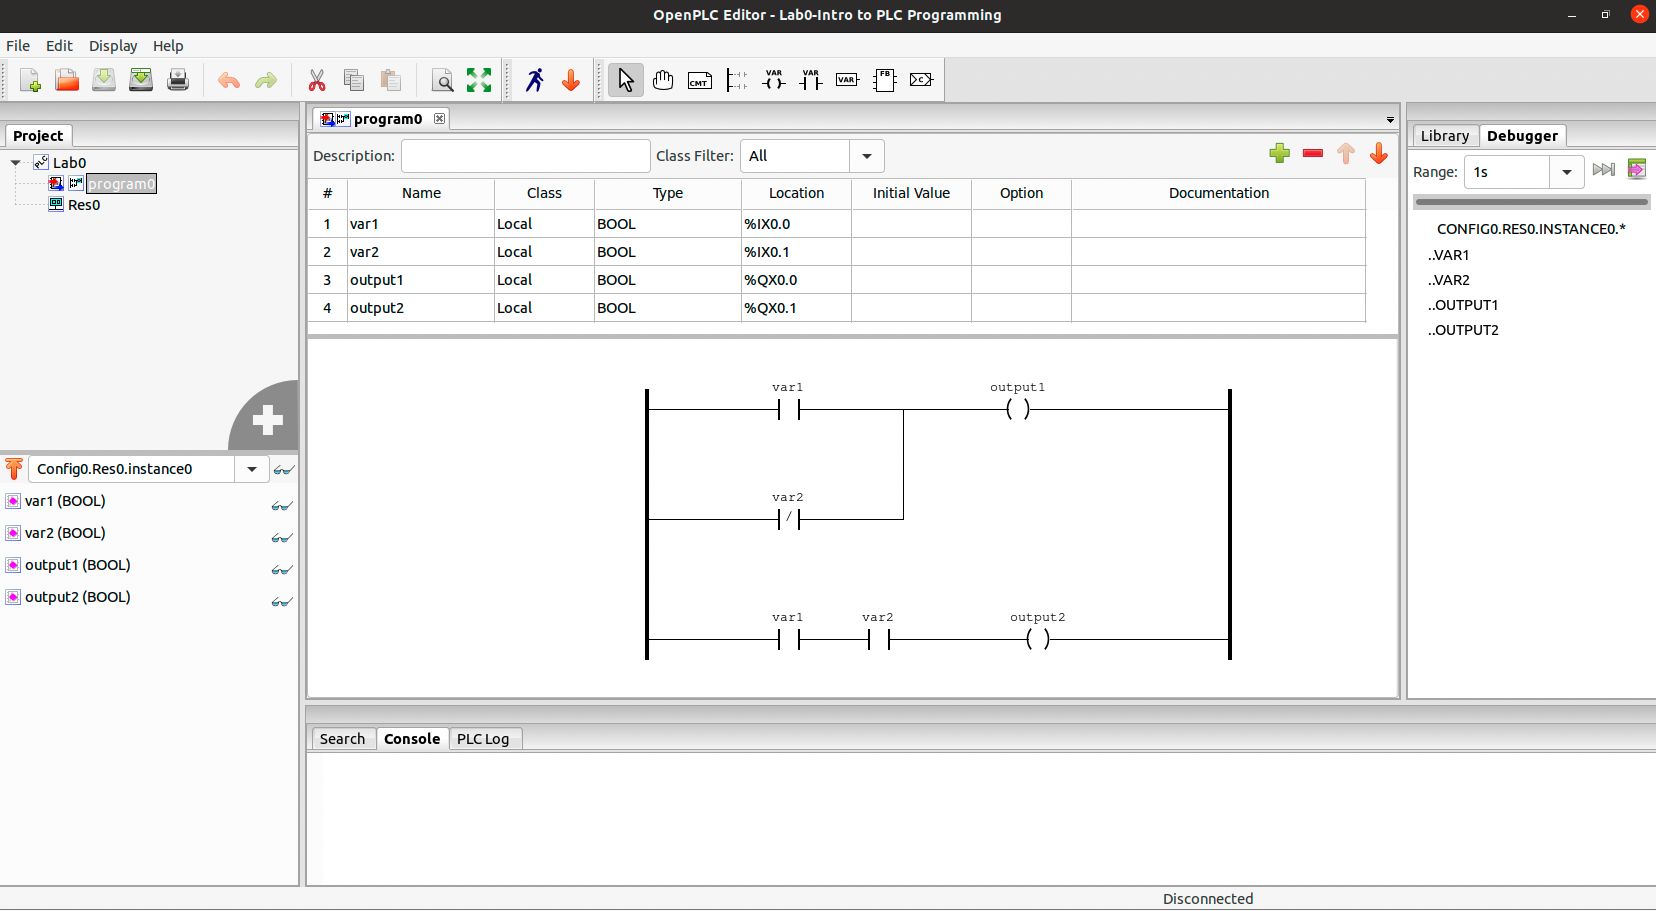
\includegraphics[width=.93\textwidth]{./images/editorProject.png}}
\end{center}
\caption{The OpenPLC Editor with a project, variable declarations and a ladder diagram}
\label{fig:editorProject}
\end{figure}

A tutorial video explaining the OpenPLC Editor, including creating projects, adding variables, creating ladder diagrams, and running the debugger can be found at [Insert URL here].


\subsection{PLC Addressing for Variables}
Figure~\ref{fig:addressing} displays a ladder diagram and the corresponding variable declarations. Normally, a PLC application interacts with the outside world through communication protocols. For the OpenPLC Editor, these interactions occur through variables.  When designing a ladder diagram, one area of consideration is which variables are available for external interaction. Any variables available for external interaction must by properly addressed in memory. The memory addressing for OpenPLC is explained below.

\begin{figure}[!htb]
\begin{center}
\tcbox[colframe=black,colback=white!30]{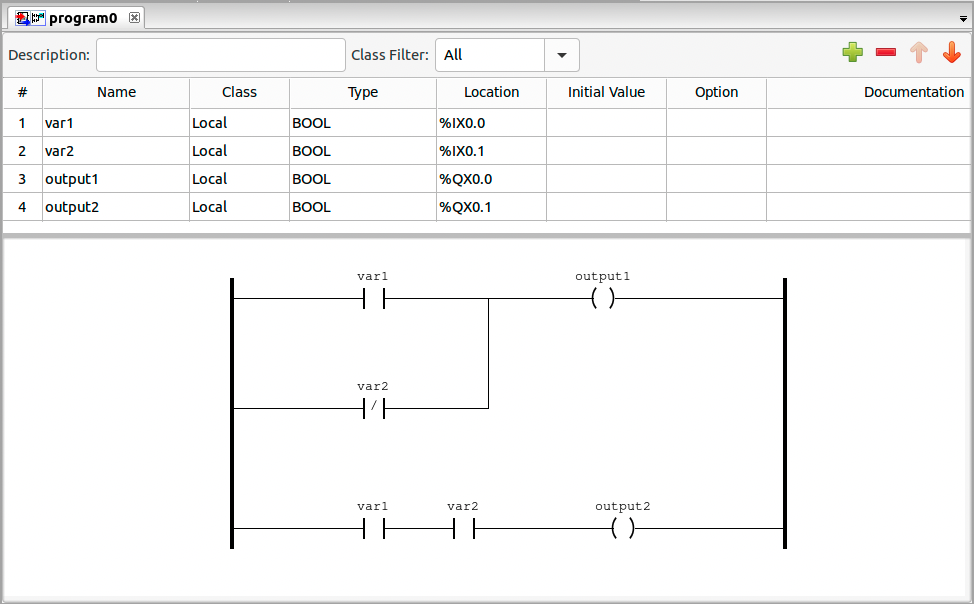
\includegraphics[width=.79\textwidth]{./images/openPLC1.png}}
\end{center}
\caption{The OpenPLC Editor with a project, variable declarations and a ladder diagram}
\label{fig:addressing}
\end{figure}

OpenPLC are composed of four ordered parts:
\begin{itemize}[noitemsep]
    \item Starts with a \% symbol.
    \item Second is the \textbf{storage class}, indicating input or output.
    \item Third is the \textbf{data size}.
    \item Forth is the \textbf{hierarchical address} location
\end{itemize}
   
The \textbf{storage class}, generally, has the following interpretation: (I) inputs, (Q) outputs, and (M) memory. The \textbf{data size} requires a data type with a predefined number of bits. OpenPLC has a set of predefined data types with corresponding sizes. 

\begin{adjustwidth}{1.5cm}{0cm}
    \begin{center}
        \textbf{Elementary Data Types and Data Sizes} \\
    \end{center}
    \begin{tabular}{|c|c|c|c|} 
    \hline 
    \textbf{Symbol} & \textbf{Data Type} & \textbf{Number of Bits} & \textbf{Elementary Data Types} \\
    \hline 
    X & Bit & 1 & BOOL\\
    \hline
    B &	Byte &	8 &	BYTE, SINT, USINT\\
    \hline
    W &	Word &	16 & WORD, INT, UINT\\
    \hline
    D &	Double Word &	32 &	DWORD, DINT, UDINT, FLOAT\\
    \hline
    L &	Long Word &	64 & LWORD, LINT, ULINT, DOUBLE\\
    \hline
    \end{tabular}
    \label{table:dataTypes}
\end{adjustwidth}



The \textbf{hierarchical address} is dependant on the data type. For a Bit the \textbf{hierarchical address}
has two-parts. The value immediately following the symbol (X) must be a number in the range  0 to 1023. After the number is a period, and then following the period must be a number in the range 0 to 7. Consider this right-most value as a position in a byte.

The \textbf{hierarchical address} for other data sizes (Byte, Word, Double Word, Long Word), the value immediately following the symbol must be a number in the range of 0 to 1023. 

\subsubsection*{Understanding Check \#3}
Given the following addresses: (1) determine which addresses are valid, (2) for the valid addresses determine the storage class, and the data type.

\begin{enumerate}[noitemsep]
    \item \%IX0.8
    \item \%IX0.1
    \item \%IB1.1
    \item \%IB11
    \item \%QB1
    \item \%QX0.0
    \item \%IX0.0
    \item \%IB1
    \item \%QD100
    \item \%ML10
\end{enumerate}
